\begin{figure}
\centering

\begin{tikzpicture}[->,>=stealth',shorten >=1pt,auto,node distance=5cm,
  thick,main node/.style={fill=white!20,draw,font=\sffamily\footnotesize\bfseries}]

  
  \node[main node] (latesRef) [ text width=2.0cm, minimum height=1.5cm, align=center]   {Reference\\(Latest)};
  \node[main node] (ctrl)     [left=0.8cm of latesRef,minimum height=2.5cm, align=center]                           {Controller};
  \node[main node] (getRef)   [right=1.5cm of latesRef, text width=3.0cm, minimum height=1.1cm, align=center]      {Get Reference};
 

 % \node[main node] (fromsim)     [above=1.0cm of getRef, text width=3.0cm, minimum height=1.1cm, align=center]    {From Simulator\\ Hold (sim mode)};
 % \node[main node] (sim)         [above=1.0cm of fromsim, text width=3.0cm, minimum height=1.1cm, align=center]    {Simulator \\Trigger\\ (sim mode)};

 \node[main node, draw=white] (haname2)   [above=0.2cm of getRef, align=center]   {};

  \node[main node] (dodebug)     [below=1.0cm of getRef, text width=3.0cm, minimum height=1.1cm, align=center]    {User Commands\\ (debug)};
  \node[main node] (tosim)       [below=1.0cm of dodebug, text width=3.0cm, minimum height=1.1cm, align=center]    {To Simulator\\ Trigger};
  \node[main node] (filter)      [below=1.0cm of tosim, text width=3.0cm, minimum height=1.1cm, align=center]     {Filter};
  \node[main node] (setRef)      [below=1.0cm of filter, text width=3.0cm, minimum height=1.1cm, align=center]    {Set Reference};
  \node[main node] (reqSens)     [below=1.0cm of setRef, text width=3.0cm, minimum height=1.1cm, align=center]    {Request Sensors};
  \node[main node] (getSens)     [below=1.0cm of reqSens, text width=3.0cm, minimum height=1.1cm, align=center]   {Get Sensors};
  \node[main node] (canWait)     [below=1.0cm of getSens, text width=3.0cm, minimum height=1.1cm, align=center]   {Wait on CAN};
  \node[main node] (putState)    [below=1.0cm of canWait, text width=3.0cm, minimum height=1.1cm, align=center]   {Put State};
  \node[main node] (rthold)      [left=0.5cm of getSens, minimum height=1.1cm, align=center]   {Real-Time\\Hold};



  \node[main node] (latestState) [left=1.5cm of putState, text width=2.0cm, minimum height=1.1cm, align=center, yshift=-1.0cm]   {State\\(Latest)};
  \node[main node, draw=white] (haname)   [right=3.0cm of putState, align=center]   {};

  \node[main node] (robot)    [right=4.8cm of getSens, minimum height=5.5cm, align=center]    {Robot};
  

%H_ref.ref[jnt] = deg;
%H_ref.mode[jnt] = HUBO_REF_MODE_ENC_FILTER;

  \path[->, dashed,every node/.style={font=\sffamily\small}]
    (ctrl) edge node [above] {} (latesRef);

%  \path[->, every node/.style={font=\sffamily\small}]
%    (fromsim) edge node [right] {$t_0=0.011~ms$} (getRef);
%\draw[->] ([xshift=-1.2 cm]fromsim.south)  to [out=-90,in=90] node [right] {$t_0=0.011~ms$} ([xshift=-1.2 cm]getRef.north)  ;
%\draw[->] ([xshift=-1.2 cm]getRef.south)   to [out=-90,in=90] node [right] {$t_1=0.011~ms$} ([xshift=-1.2 cm]tosim.north)  ;
%\draw[->] ([xshift=-1.2 cm]tosim.south)   to [out=-90,in=90] node [right] {$t_2=0.011~ms$} ([xshift=-1.2 cm]filter.north)  ;
%\draw[->] ([xshift=-1.2 cm]filter.south)   to [out=-90,in=90] node [right] {$t_3=???~ms$} ([xshift=-1.2 cm]setRef.north)  ;
%\draw[->] ([xshift=-1.2 cm]setRef.south)   to [out=-90,in=90] node [right] {$t_4=???~ms$} ([xshift=-1.2 cm]reqSens.north)  ;
%\draw[->] ([xshift=-1.2 cm]reqSens.south)   to [out=-90,in=90] node [right] {$t_5=???~ms$} ([xshift=-1.2 cm]getSens.north)  ;
%\draw[->] ([xshift=-1.2 cm]getSens.south)   to [out=-90,in=90] node [right] {$t_6=0.011~ms$} ([xshift=-1.2 cm]putState.north)  ;
%\draw[->] ([xshift=0.0 cm]putState.west)   to [out=180,in=-90] node [below, yshift=-0.5cm, xshift=-0.2cm] {$t_7=0.011~ms$} ([xshift=0.0 cm]rthold.south)  ;


\draw[->] ([xshift=0.0cm]latesRef.east)  to [out=0,in=-180]  node [right]  {} ([xshift=0.0cm]getRef.west)  ;
%\draw[->] ([xshift=0.0cm]fromsim.south)  to [out=-90,in=90]  node [right]  {} ([xshift=0.0cm]getRef.north)  ;
\draw[->] ([xshift=0.0cm]getRef.south)   to [out=-90,in=90]  node [right]  {} ([xshift=0.0cm]dodebug.north)  ;
\draw[->] ([xshift=0.0cm]dodebug.south)  to [out=-90,in=90]  node [right]  {} ([xshift=0.0cm]tosim.north)  ;
\draw[->] ([xshift=0.0cm]tosim.south)    to [out=-90,in=90]  node [right]  {} ([xshift=0.0cm]filter.north)  ;
\draw[->] ([xshift=0.0cm]filter.south)   to [out=-90,in=90]  node [right]  {} ([xshift=0.0cm]setRef.north)  ;
\draw[->] ([xshift=0.0cm]setRef.south)   to [out=-90,in=90]  node [right]  {} ([xshift=0.0cm]reqSens.north)  ;
\draw[->] ([xshift=0.0cm]reqSens.south)  to [out=-90,in=90]  node [right]  {} ([xshift=0.0cm]getSens.north)  ;
\draw[->] ([xshift=0.0cm]getSens.south)  to [out=-90,in=90]  node [right]  {} ([xshift=0.0cm]canWait.north)  ;
\draw[->] ([xshift=0.0cm]canWait.south)  to [out=-90,in=90]  node [right]  {} ([xshift=0.0cm]putState.north)  ;
\draw[->] ([xshift=0.0 cm]putState.west) to [out=180,in=-90] node [below, yshift=-0.5cm, xshift=-0.2cm] {} ([xshift=0.0 cm]rthold.south)  ;
\draw[->] ([xshift=0.0 cm]rthold.north)  to [out=90,in=-120] node [left, yshift=-1.0cm, xshift=-0.8cm, rotate=90] {} ([xshift=0.0 cm]getRef.west)  ;
\draw[->] ([xshift=0.0cm]putState.south) to [out=-90,in=0]   node [right]  {} ([xshift=0.0cm]latestState.east)  ;




%\draw[->] ([yshift=0.75cm]fromsim.east)  to [out=-30,in=30] node [right] {$t_0=0.014~ms$} ([yshift=-0.75cm]fromsim.east)  ;
\draw[->] ([yshift=0.75cm]getRef.east)  to [out=-30,in=30] node [right] {$t_0=0.010~ms$} ([yshift=-0.75cm]getRef.east)  ;
\draw[->] ([yshift=0.75cm]dodebug.east)  to [out=-30,in=30] node [right] {$t_1=0.011~ms$} ([yshift=-0.75cm]dodebug.east)  ;
\draw[->] ([yshift=0.75cm]tosim.east)  to [out=-30,in=30] node [right] {$t_2=0.014~ms$} ([yshift=-0.75cm]tosim.east)  ;
\draw[->] ([yshift=0.75cm]filter.east)  to [out=-30,in=30] node [right] {$t_3=0.008~ms$} ([yshift=-0.75cm]filter.east)  ;
\draw[->] ([yshift=0.75cm]setRef.east)  to [out=-30,in=30] node [right] {$t_4=0.152~ms$} ([yshift=-0.75cm]setRef.east)  ;
\draw[->] ([yshift=0.75cm]reqSens.east)  to [out=-47,in=47] node [right] {$t_5=1.365~ms$} ([yshift=-0.75cm]getSens.east)  ;
\draw[->] ([yshift=0.75cm]canWait.east)  to [out=-30,in=30] node [right,align=center] {$t_6=3.000~ms$\\(hard timeout)} ([yshift=-0.75cm]canWait.east)  ;
%\draw[->] ([yshift=0.75cm]reqSens.east)  to [out=-30,in=30] node [right] {$t_5=???~ms$} ([yshift=-0.75cm]reqSens.east)  ;
%\draw[->] ([yshift=0.75cm]getSens.east)  to [out=-30,in=30] node [right] {$t_6=???~ms$} ([yshift=-0.75cm]getSens.east)  ;
\draw[->] ([yshift=0.75cm]putState.east)  to [out=-30,in=30] node [right] {$t_7=0.092~ms$} ([yshift=-0.75cm]putState.east)  ;
\draw[->] ([yshift=-0.75cm]rthold.west)  to [out=120,in=-120] node [above, yshift=1.5cm, xshift=0.3cm, rotate=90] {$\displaystyle t_{hold}=T-\sum_{i=0}^{8} t_i=0.348~ms$} ([yshift=0.75cm]rthold.west)  ;

\draw[->, dashed] ([xshift=0.0cm]latestState.west)   to [out=120,in=-90] node [right] {} ([xshift=0.0cm]ctrl.south)  ;
%\draw[->, dashed] ([xshift=0.0cm]sim.south)   to [out=-90,in=90] node [right] {} ([xshift=0.0cm]fromsim.north)  ;

\node[fit=(getRef)(putState)(rthold)(haname)(latestState)(haname2), draw,label={south:Hubo-Ach}] (hubo-ach) [minimum width=4.5cm] {};



\draw[->,loosely dotted] ([xshift=0.75cm]setRef.south)  to [out=-30,in=-180] node [above] {} ([yshift=1.50cm]robot.west)  ;
\draw[->,loosely dotted] ([xshift=0.75cm]reqSens.south)  to [out=-30,in=-180] node [above] {} ([yshift=0.75cm]robot.west)  ;
\draw[<-,loosely dotted] ([xshift=0.0cm]getSens.east)  to [out=0,in=-180] node [above, xshift=1.7cm] {CAN} ([yshift=0.0cm]robot.west)  ;
\draw[<-,loosely dotted] ([xshift=0.75cm]canWait.north)  to [out=30,in=-180] node [above] {} ([yshift=-0.75cm]robot.west)  ;




%  \path[->,every node/.style={font=\sffamily\small}]
%    (ik) edge node [above] {$\overline{\theta_d}$} (filter);

% \draw[->] ([xshift=-0.5 cm]filter.south)  -- node [left] {$\overline{\theta_r}$} ([xshift=-0.5 cm]hubo-ach.north)  ;
% \draw[->] ([xshift=0.5 cm]hubo-ach.north) -- node [left] {$\overline{\theta_a}$} ([xshift=0.5 cm]filter.south)  ;

% \path[<->,dashed, every node/.style={font=\sffamily\small}]
%    (hubo) edge node [above] {CAN} (hubo-ach);


\end{tikzpicture}
\caption{Timing diagram of Hubo-Ach.  All times $t_*$ denote measured times each block takes to complete.  Tests were done on a 1.6Ghz Atom D525 Dual Core with 1GB DDR3 800Mhz memory running Ubuntu 12.04 LTS linux kernel 3.2.0-29 on a Hubo2+ utilizing a CAN bus running at 1Mbps baud.  Average CPU usage is 7.6\% using a total of 4Mb or memory.}
\label{fig:hubo-ach-timing}
\end{figure}


To ensure that the Hubo-Ach controller is able to run at the desired control rates, timing experiments of each part of the controller was taken.
All tests were done with a sample step size of $0.005~sec$.
Each of the following figures have the same X and Y scale.
This is to give a visual representation of how much each portion of the cycle each part of Hubo-Ach takes up.




Fig.~\ref{fig:timing-getRef} shows the amount of time it takes to request and get the reference for the actuators.
This reads the most recent reference off of the feedforward channel and uses that as the reference used in this cycle of Hubo-Ach.
This time is measured to be $0.0010~ms$ with micro-second accuracy.
The standard deviation is $0.0028$.



Fig.~\ref{fig:timing-doCmd} shows the amount of time it takes to complete all unread commands given by the user via the console.
User commands are manual actions such as homing individual or all joints, resetting actuator errors, and reading error states.
This time is measured to be $0.011~ms$ with micro-second accuracy.
The standard deviation is $0.0.0033$.


Fig.~\ref{fig:timing-getTrigger} shows the amount of time it takes to send the external trigger.  
This external trigger tells a controller or simulator when the new reference's and commands have been read.
In real-time mode the measured time delay is $0.0014~ms$ with micro-second accuracy and a standard deviation of $0.0035$.


Fig.~\ref{fig:timing-filter} shows the amount of time it takes to process the built in filter.
This filter has multiple options:
\begin{itemize}
\item Direct reference mode where the filter acts as a reference pass through (Section~\ref{sec:singlejointStep}.
\item Low pass filter based on previous reference commands (Section~\ref{sec:singlejointFilter}.
\item Low pass filter using feedback from the actual position of the joint (Section~\ref{sec:singlejointEnc}).
\item Compliance amplification mode which artificially increases the compliance of the joint (Section~\ref{sec:singlejointRefComplience})
The measured time delay is $0.0080~ms$ with micro-second accuracy.
The standard deviation is $0.0030~ms$.





Fig.~\ref{fig:timing-getPos} The amount of time it takes to request and get the actual position from the actuators.





\begin{figure}[thpb]
  \centering
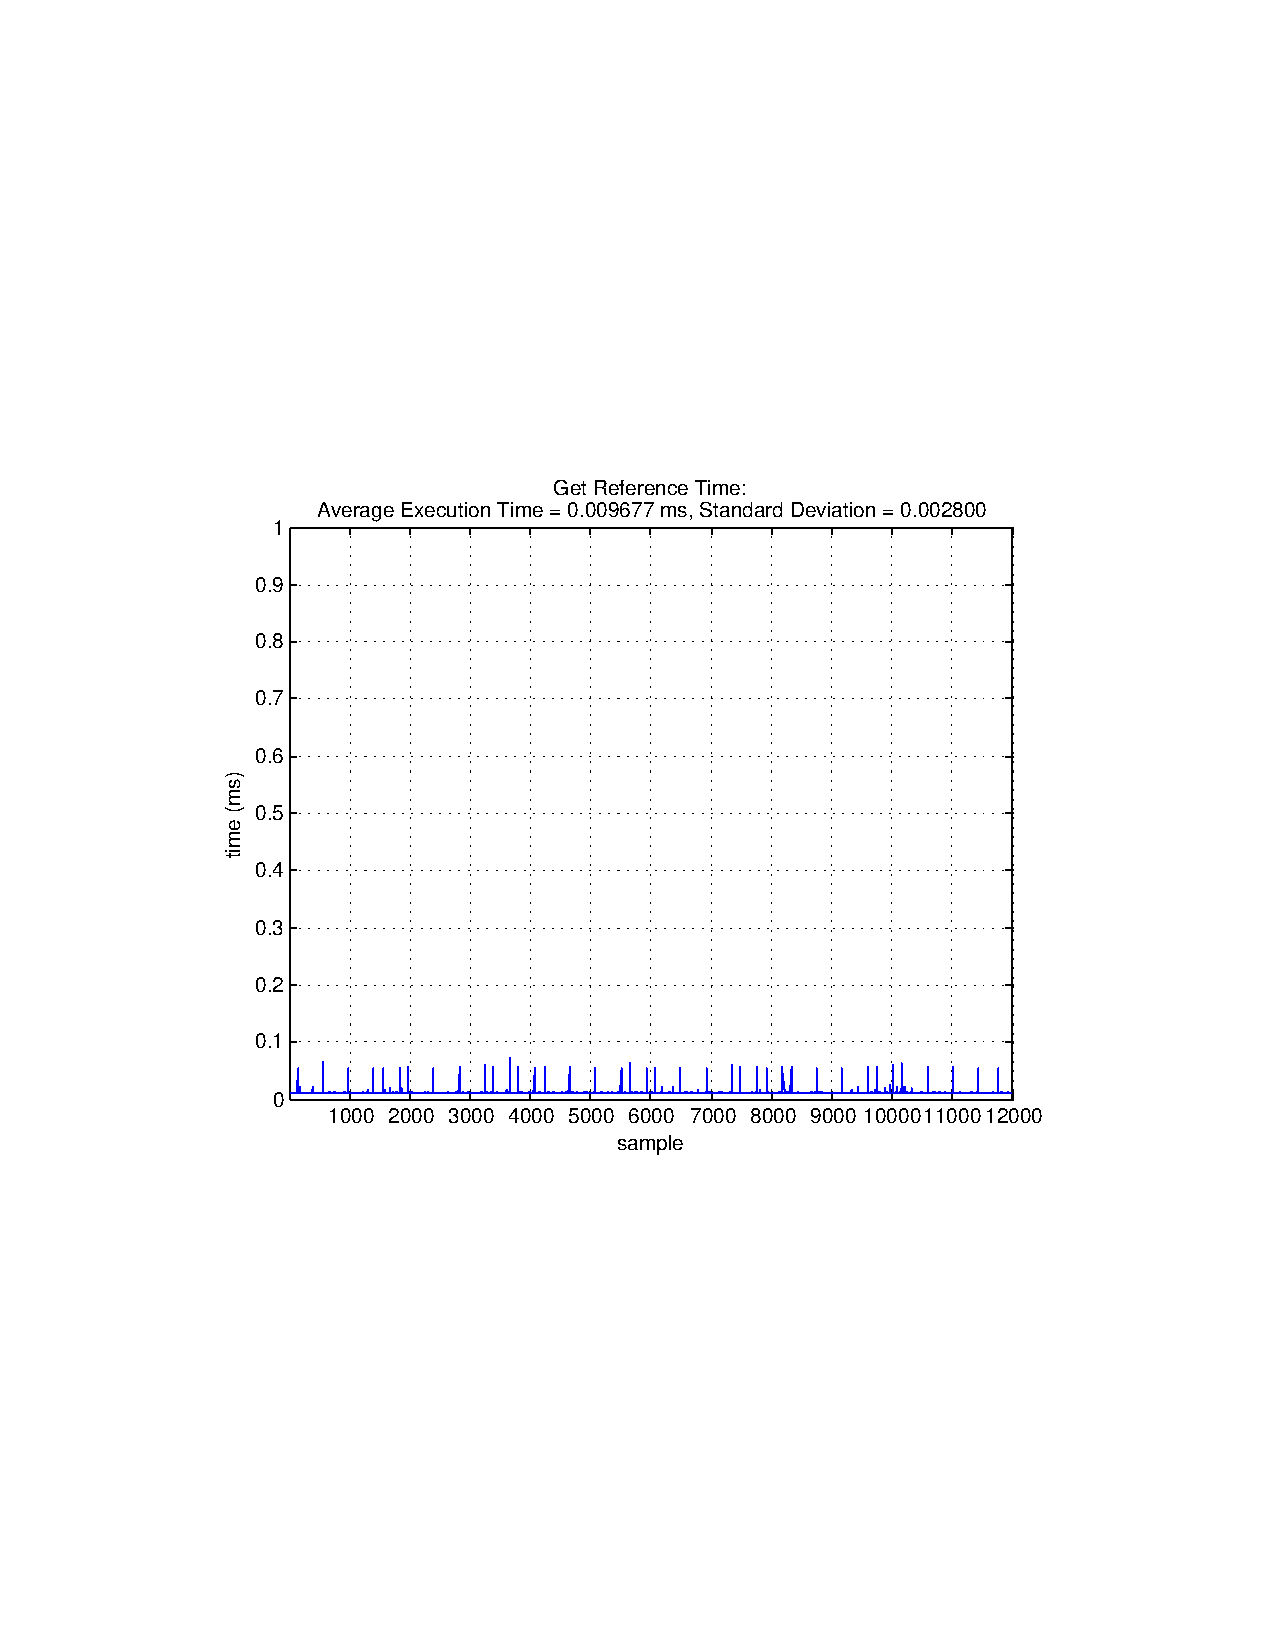
\includegraphics[width=0.6\columnwidth]{./timingData/getRef.pdf}
  \caption{The amount of time it takes to request and get the reference for the actuators.  In this case each sample has a time step of $0.005~sec$}
  \label{fig:timing-getRef}
\end{figure}


\begin{figure}[thpb]
  \centering
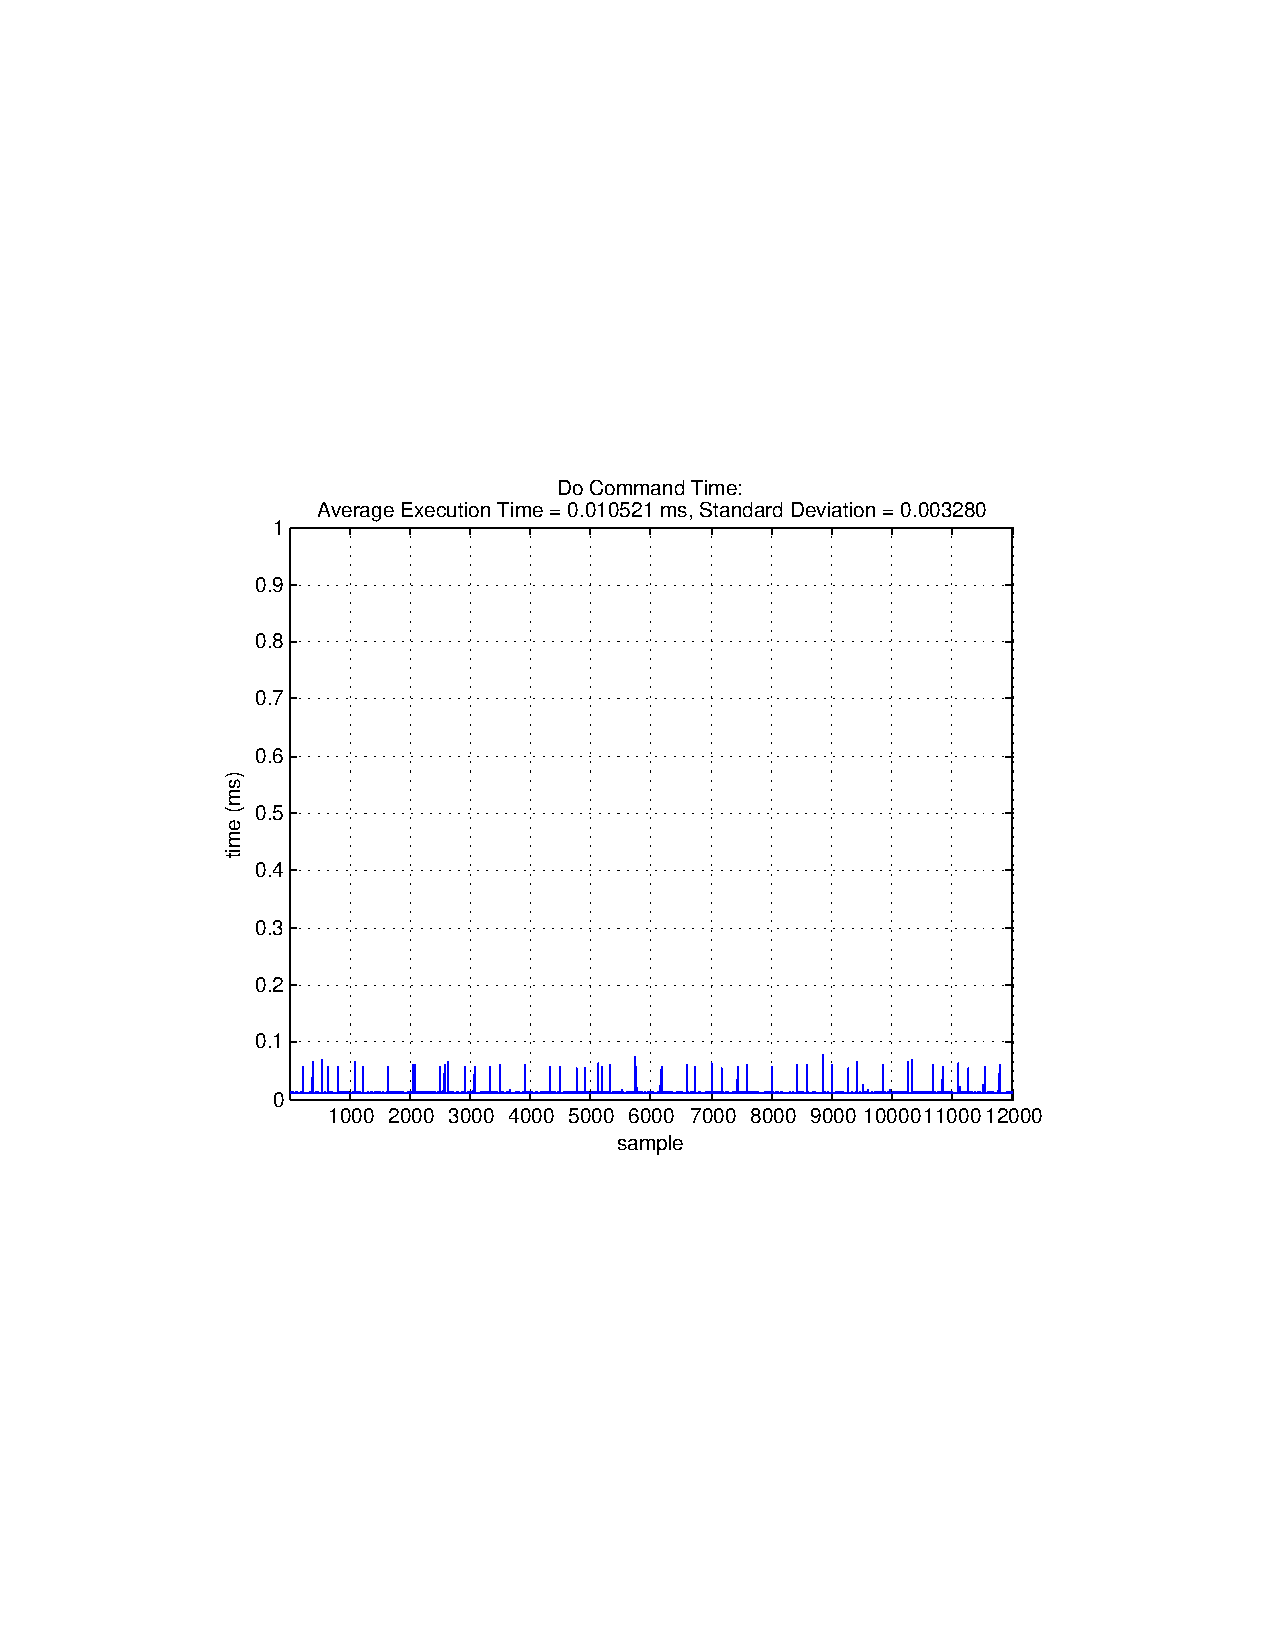
\includegraphics[width=0.6\columnwidth]{./timingData/doCmd.pdf}
  \caption{The amount of time it takes to complete all unread commands given by the user via the console.  In this case each sample has a time step of $0.005~sec$}
  \label{fig:timing-doCmd}
\end{figure}


\begin{figure}[thpb]
  \centering
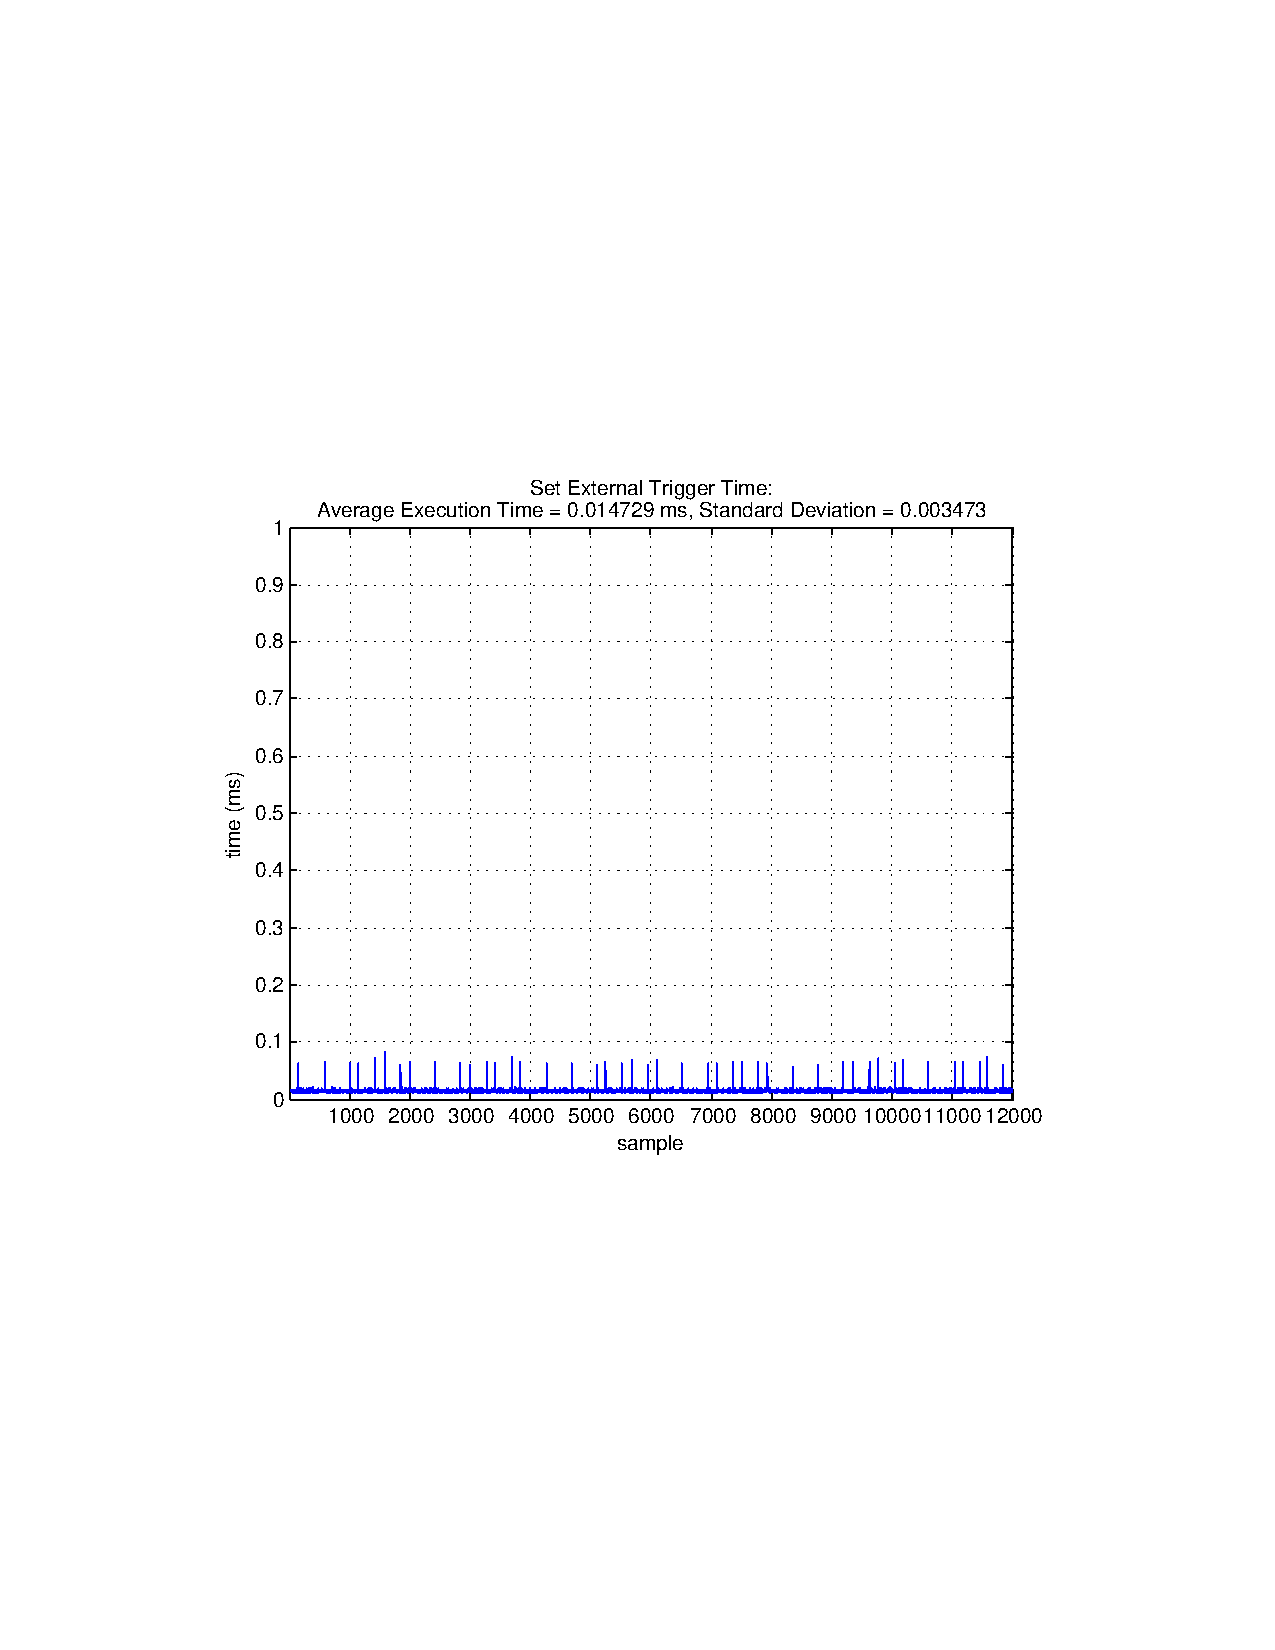
\includegraphics[width=0.6\columnwidth]{./timingData/getTrigger.pdf}
  \caption{The amount of time it takes to send the external trigger.  In this case each sample has a time step of $0.005~sec$}
  \label{fig:timing-getTrigger}
\end{figure}

\begin{figure}[thpb]
  \centering
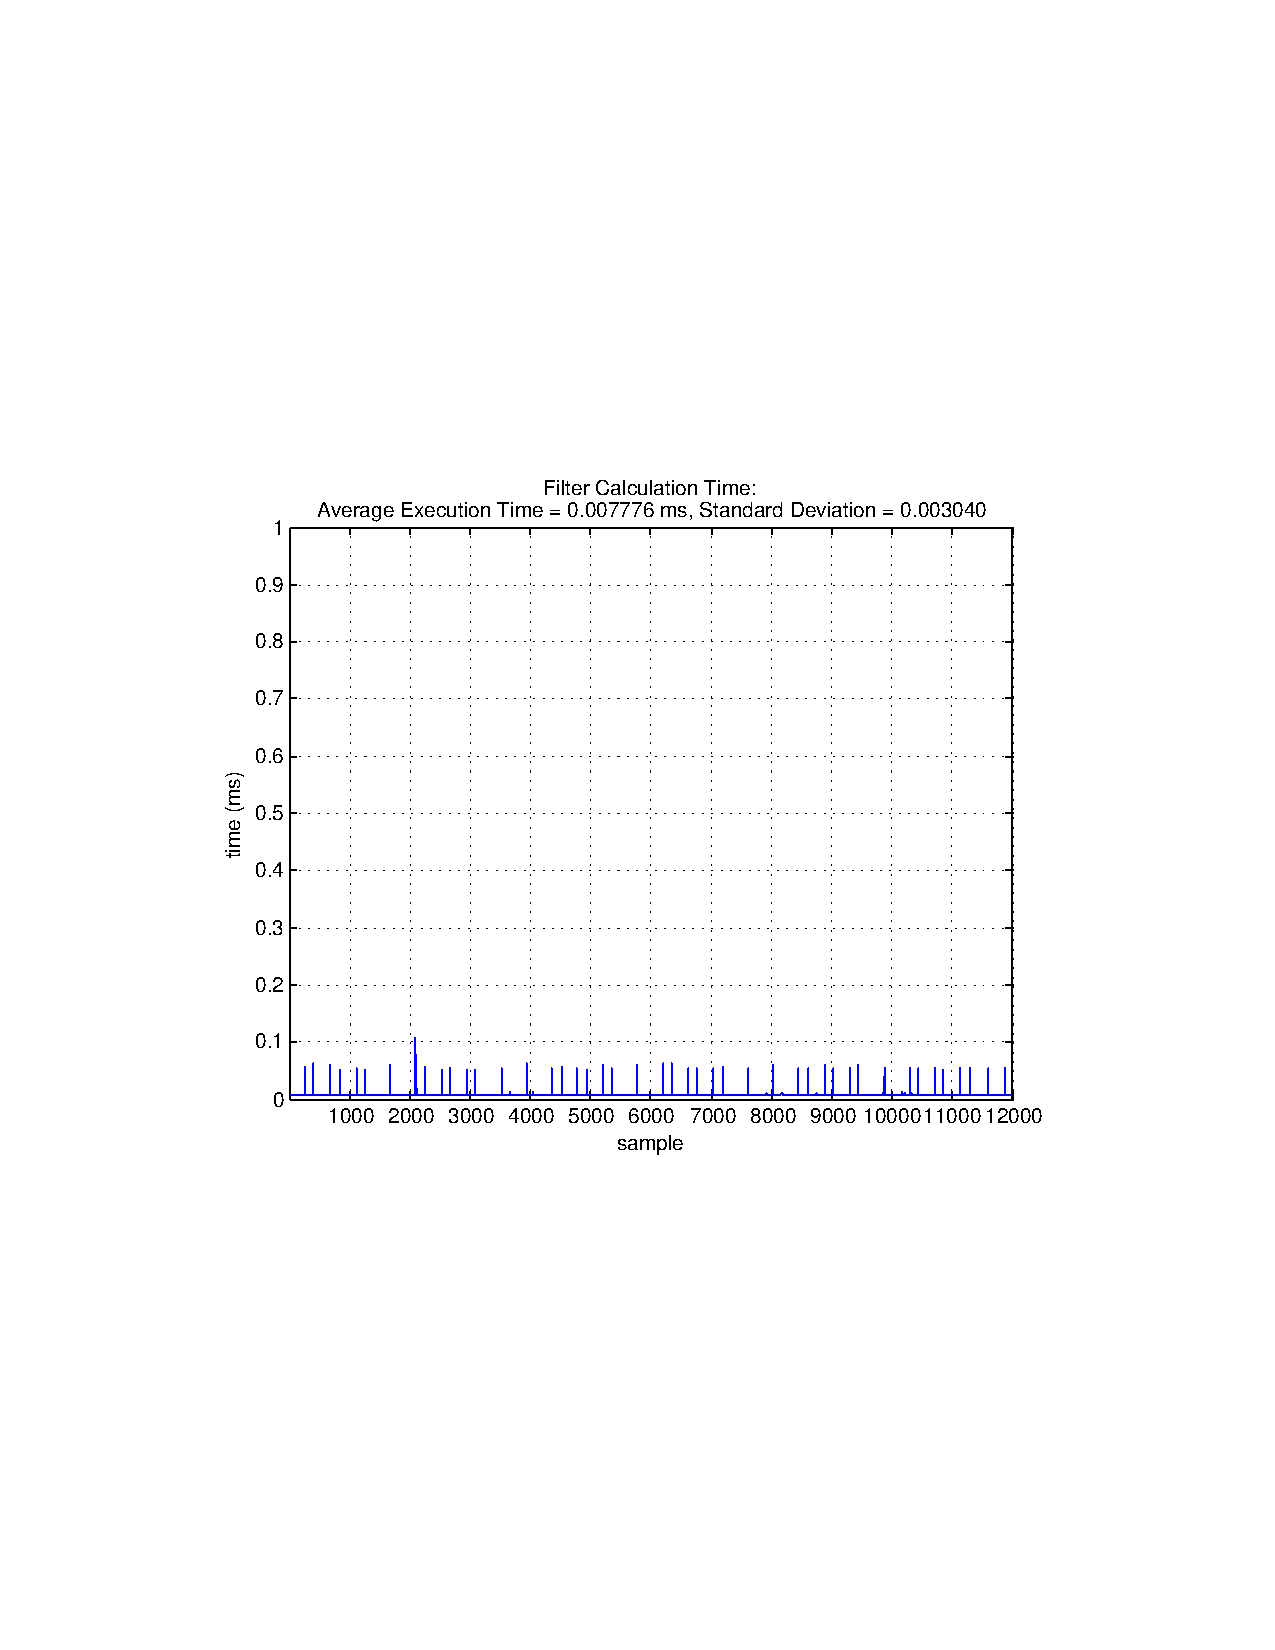
\includegraphics[width=0.6\columnwidth]{./timingData/filter.pdf}
  \caption{The amount of time it takes to process the built in filter.  In this case each sample has a time step of $0.005~sec$}
  \label{fig:timing-filter}
\end{figure}










\begin{figure}[thpb]
  \centering
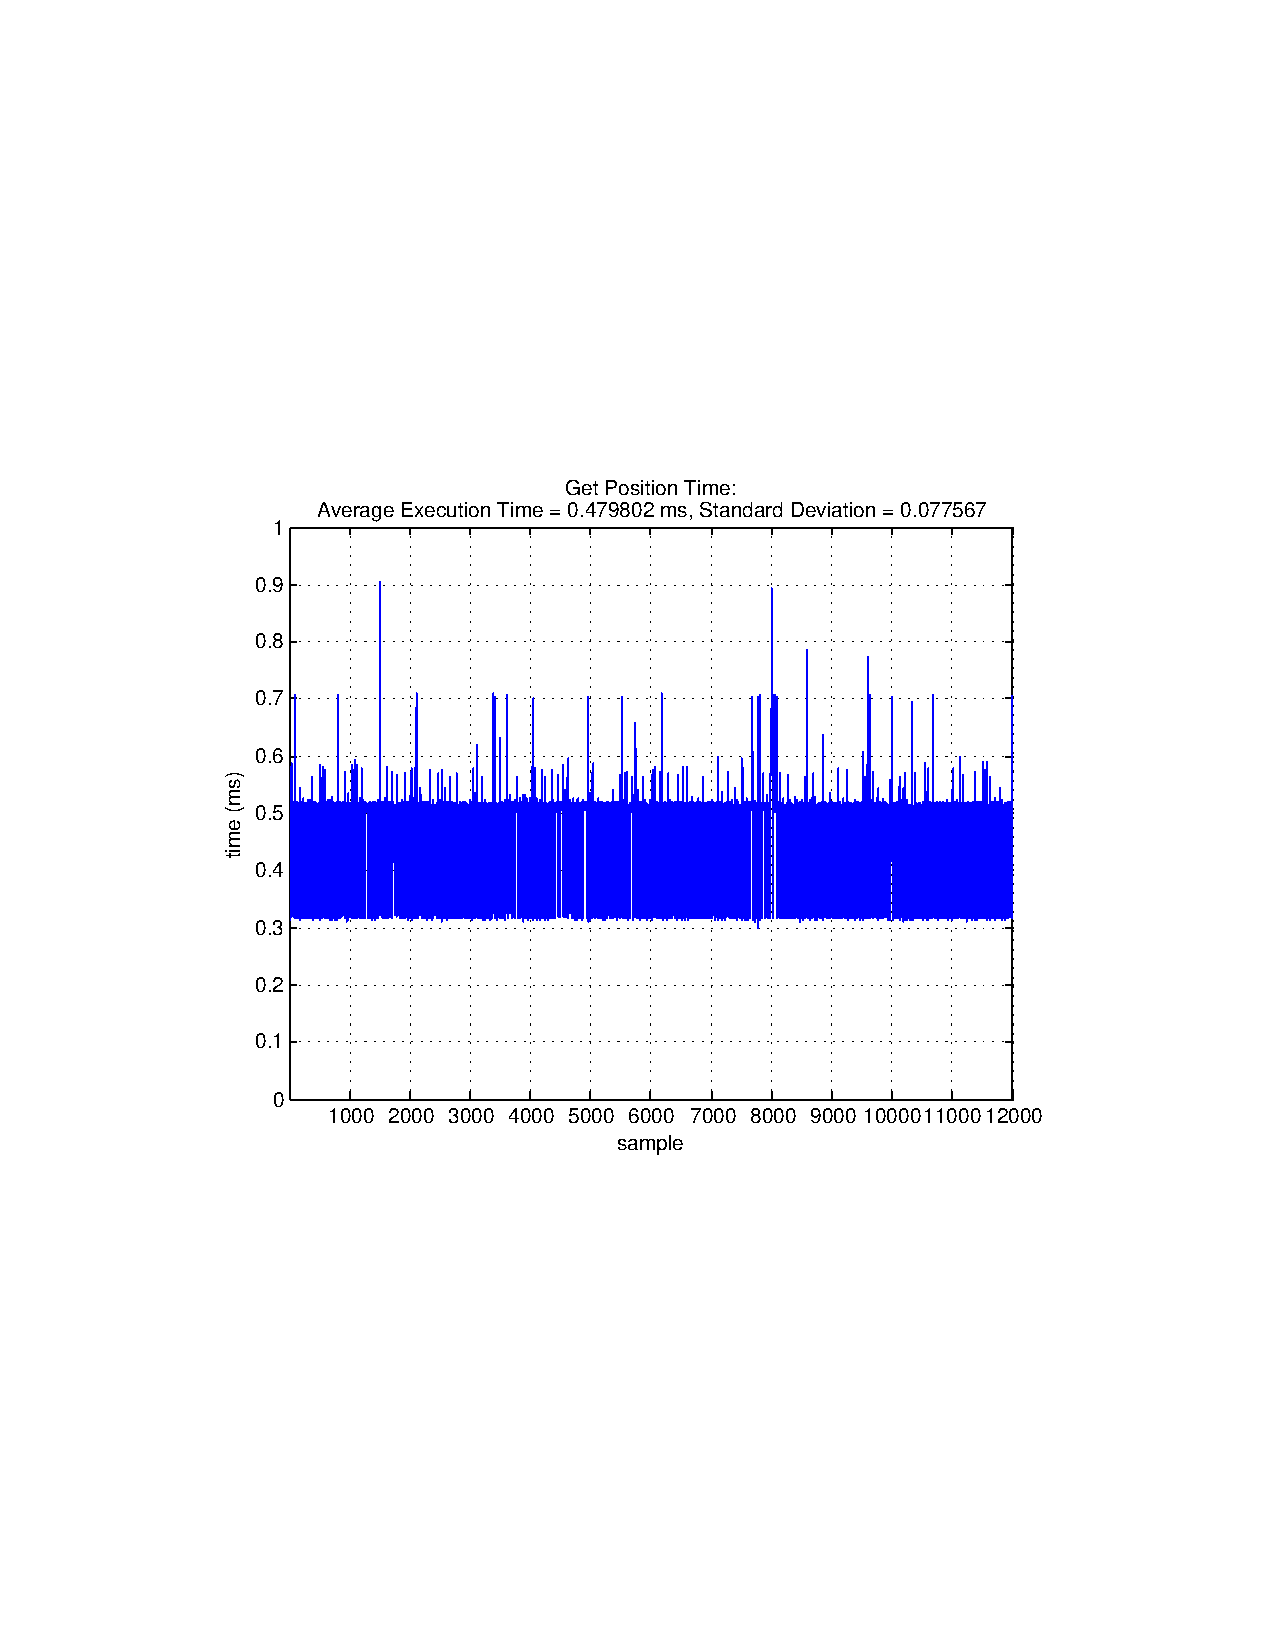
\includegraphics[width=0.6\columnwidth]{./timingData/getPos.pdf}
  \caption{The amount of time it takes to request and get the actual position from the actuators.  In this case each sample has a time step of $0.005~sec$}
  \label{fig:timing-getPos}
\end{figure}

\begin{figure}[thpb]
  \centering
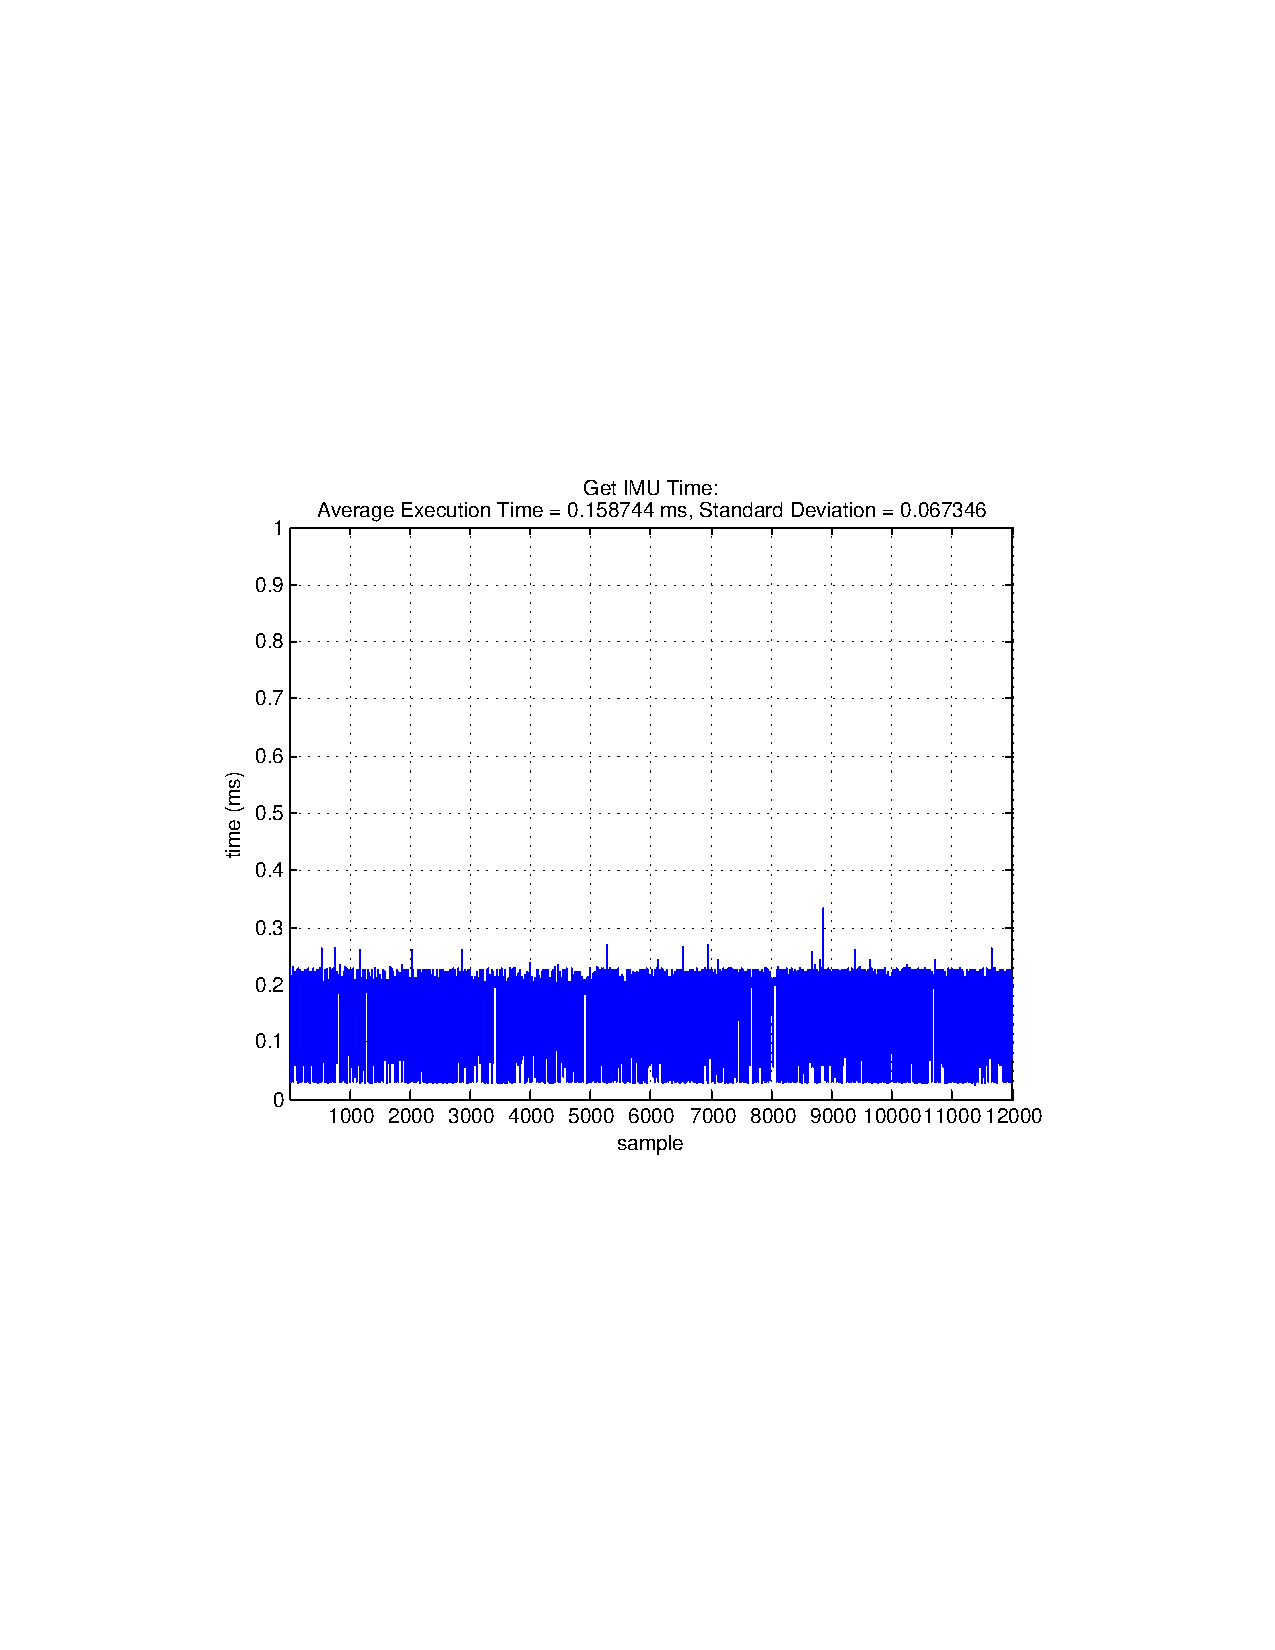
\includegraphics[width=0.6\columnwidth]{./timingData/getImu.pdf}
  \caption{The amount of time it takes to request and get the IMU data.  In this case each sample has a time step of $0.005~sec$}
  \label{fig:timing-imu}
\end{figure}


\begin{figure}[thpb]
  \centering
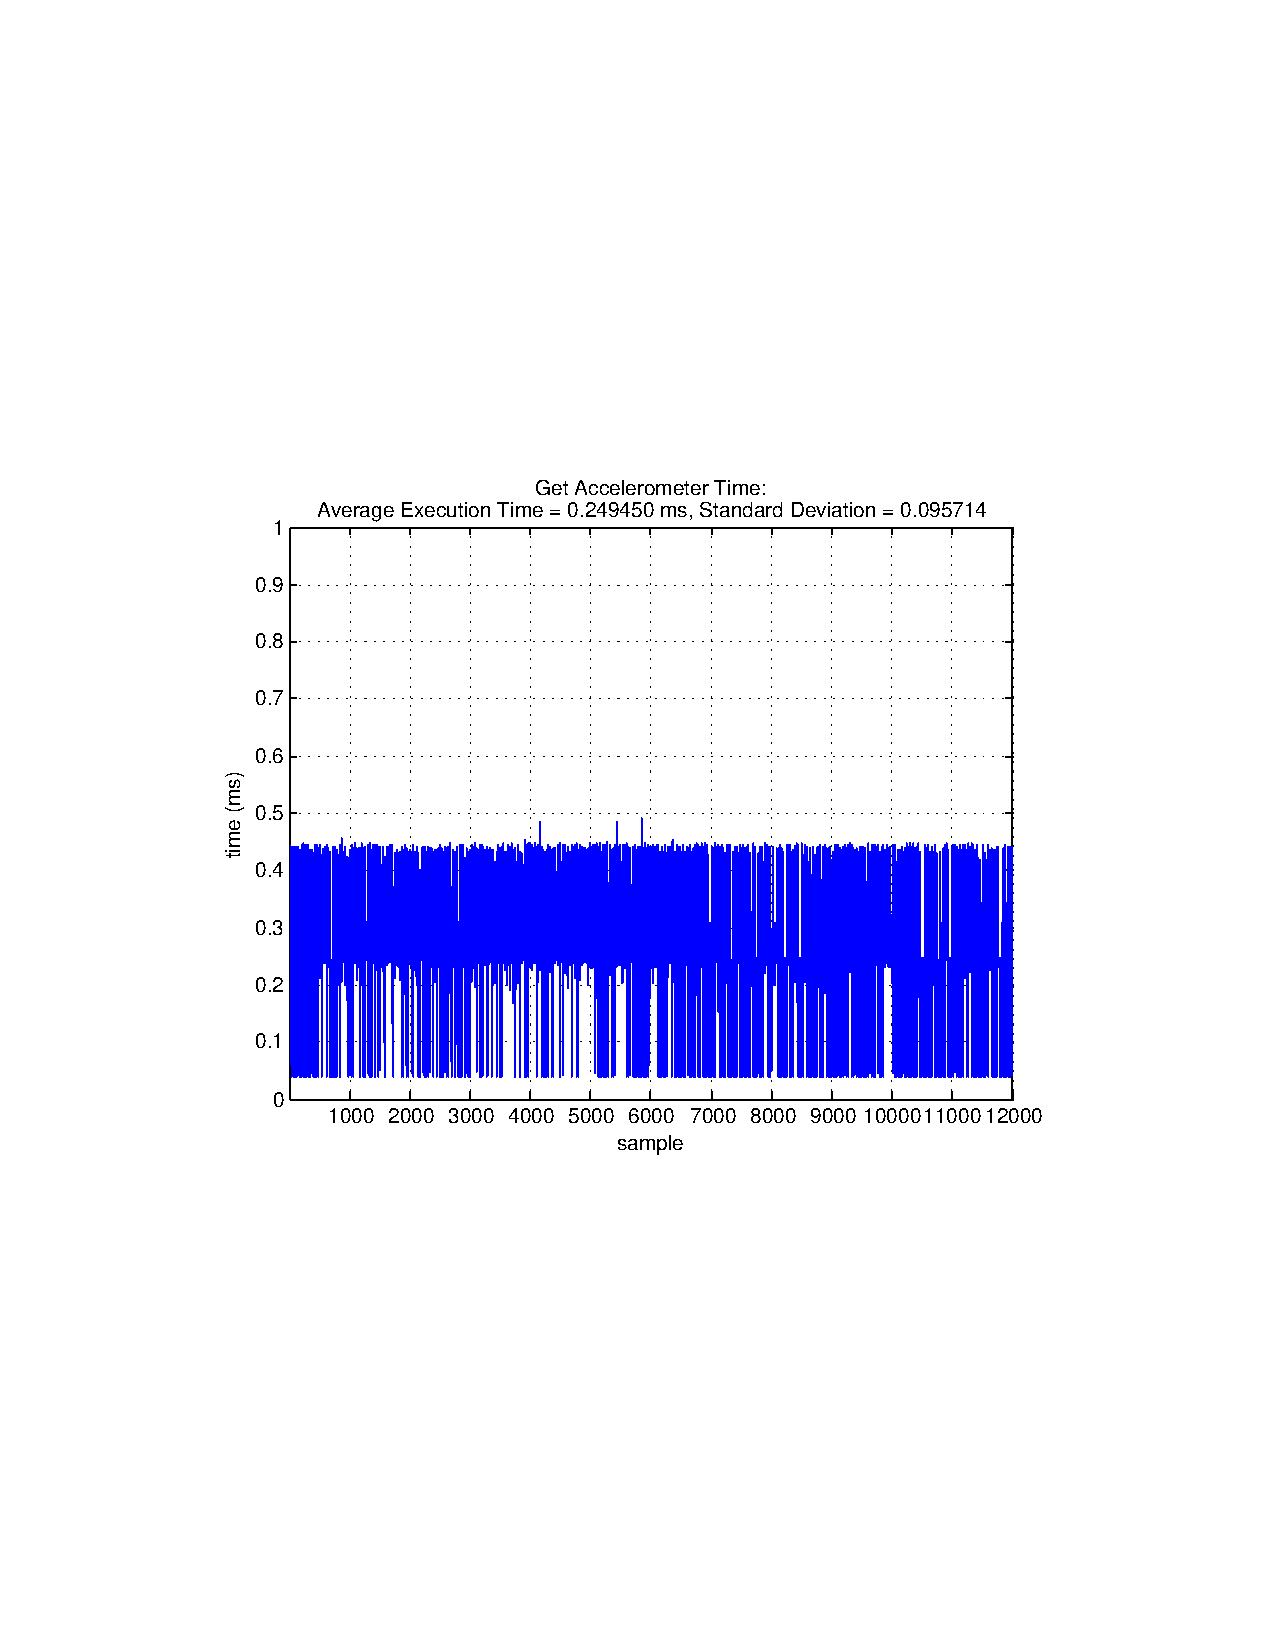
\includegraphics[width=0.6\columnwidth]{./timingData/getAcc.pdf}
  \caption{The amount of time it takes to request and get the accelerometers data.  In this case each sample has a time step of $0.005~sec$}
  \label{fig:timing-acc}
\end{figure}



\begin{figure}[thpb]
  \centering
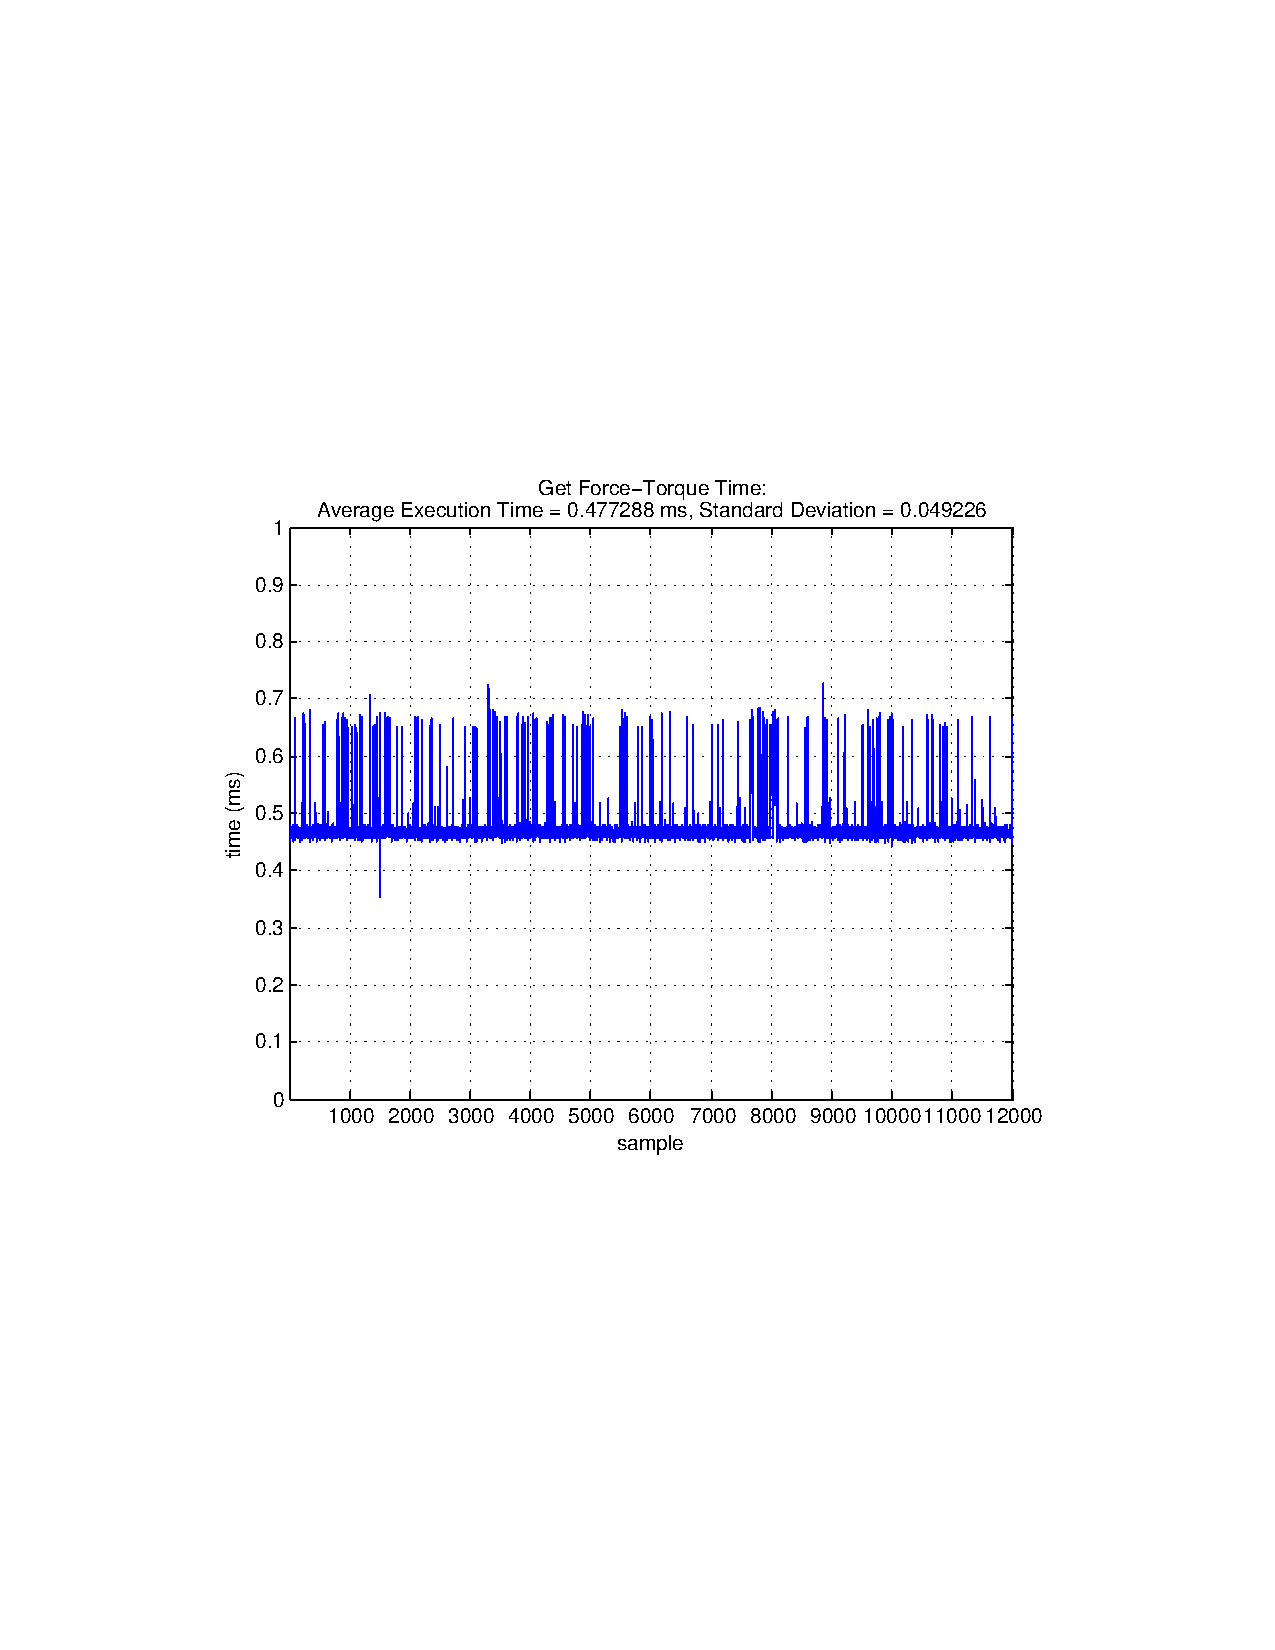
\includegraphics[width=0.6\columnwidth]{./timingData/getFt.pdf}
  \caption{The amount of time it takes to request and get the force-torque sensors.  In this case each sample has a time step of $0.005~sec$}
  \label{fig:timing-ft}
\end{figure}














\begin{figure}[thpb]
  \centering
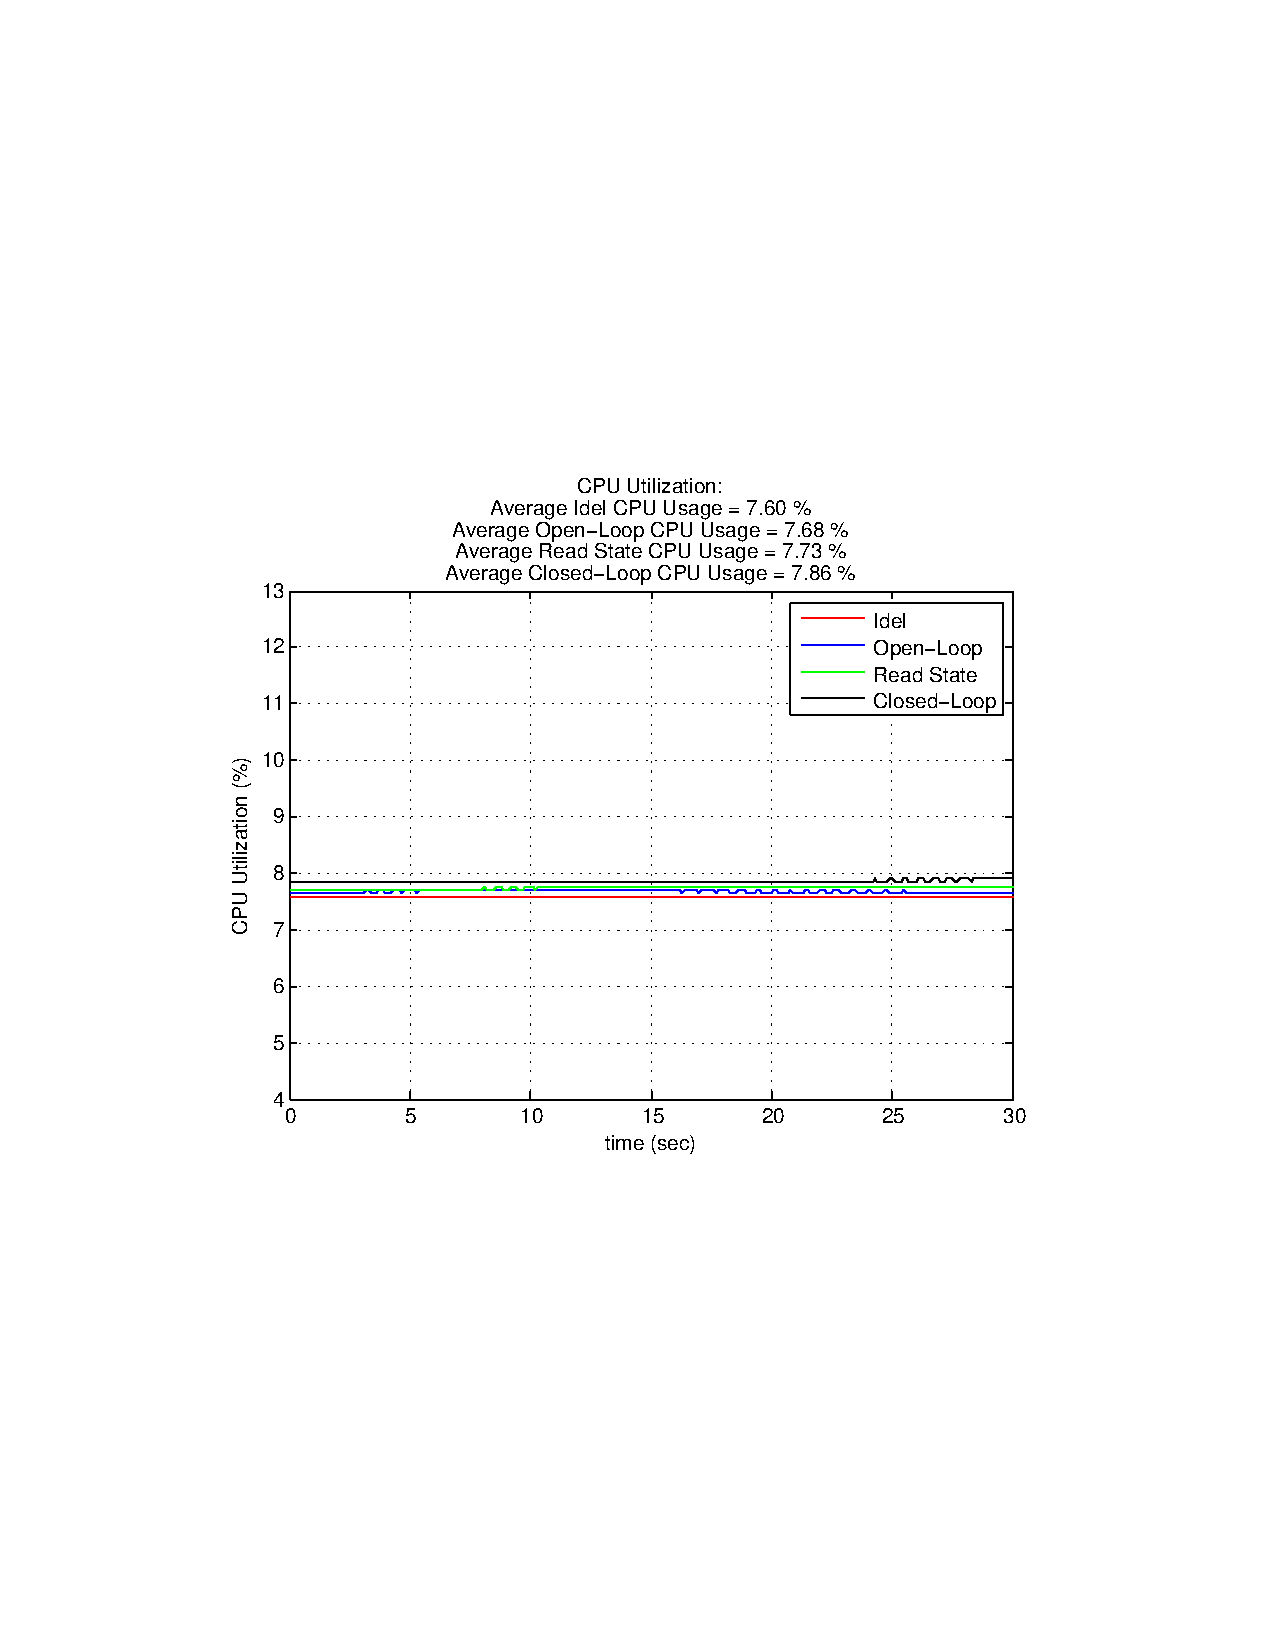
\includegraphics[width=0.6\columnwidth]{./timingData/cpu.pdf}
  \caption{CPU utilization for the Hubo-Ach process when 1) idle, 2) under open-loop control, 3) reading the sensors, and 4) under closed-loop control.  
It is important to note that the cpu utilization stays within 0.3\% when idle and under closed loop control.
This means that the CPU utilization of Hubo-Ach is independent of the external control method.
Thus it will not add more to the CPU load under complex control schemes then under simple ones.}
  \label{fig:timing-getTrigger}
\end{figure}

